\chapter{Supplemental for Chapter \refchC}
%\counterwithin{figure}{section}
%\beginsupplement

\begin{figure}[H]
% TODO: rip this out?
\centering
    % Original:
    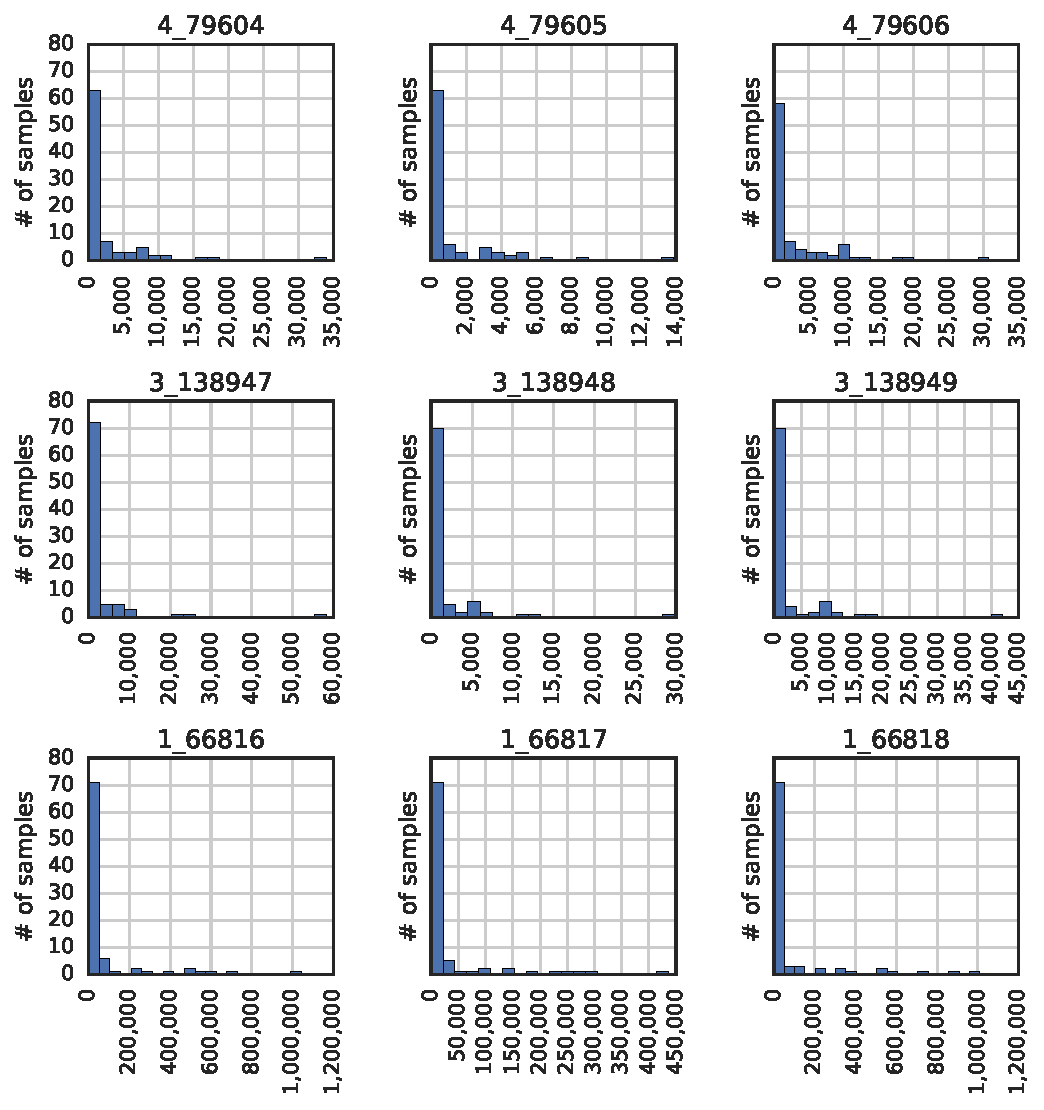
\includegraphics[width=0.8\textwidth]{./tex/chapter3/figures/170403_read_count_distributions--3_pmoCAB_clusters.pdf}
    \begin{singlespace}
    \caption[]{
        Histograms of read counts for three sets of \textit{pmoCAB} gene clusters.
        These data do not represent normal distributions.
        }
    \label{fig:pmoCAB_expressions}
    \end{singlespace}
\end{figure}


\begin{figure}[H]
\centering
    %
    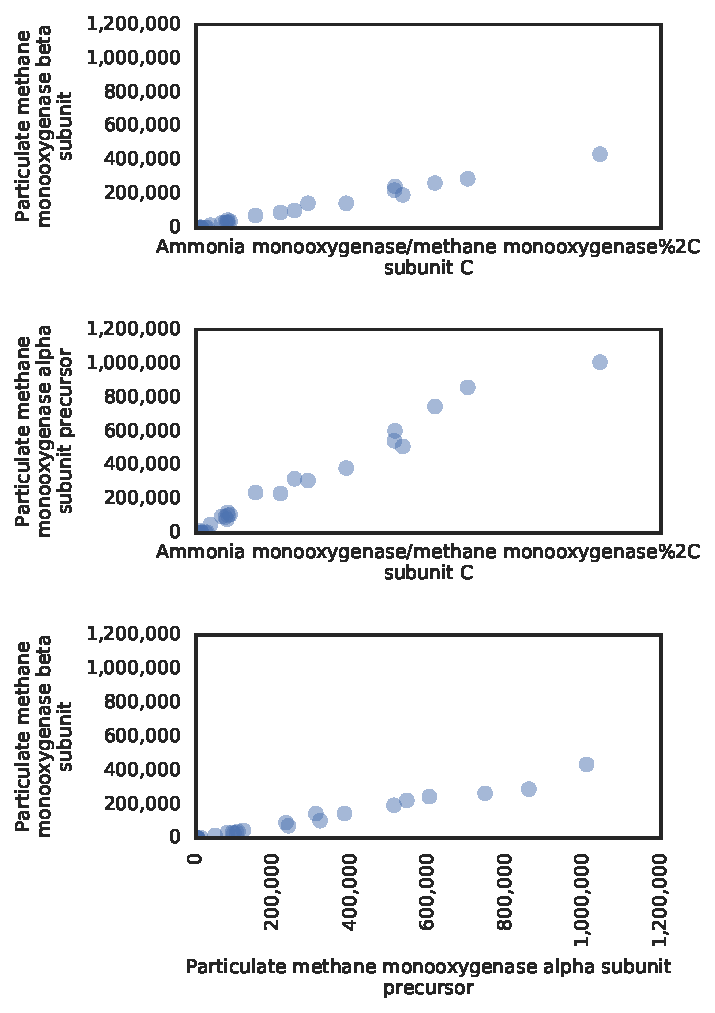
\includegraphics[width=0.6\textwidth]{./tex/chapter3/figures/170402_correlations_between_pMMO_subunits--set1.pdf}
    \begin{singlespace}
    \caption[Demonstration of correlation between \textit{pmo} subniuts in cluster 1]{
        Demonstration of correlation between \textit{pmo} subniuts in cluster 1.}
    \label{fig:pmo_cor1}
    \end{singlespace}
\end{figure}

\begin{figure}[H]
\centering
    %
    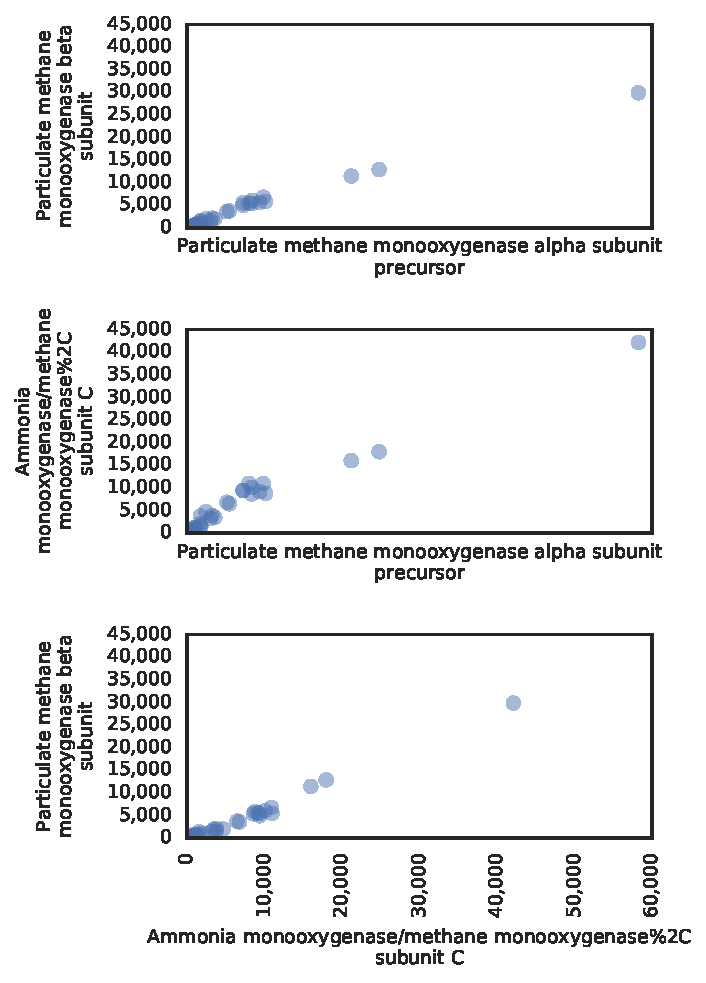
\includegraphics[width=0.7\textwidth]{./tex/chapter3/figures/170402_correlations_between_pMMO_subunits--set2.pdf}
    \begin{singlespace}
    \caption[Demonstration of correlation between \textit{pmo} subniuts in cluster 2]{
        Demonstration of correlation between \textit{pmo} subniuts in cluster 2.}
    \label{fig:pmo_cor2}
    \end{singlespace}
\end{figure}

\begin{figure}[H]
\centering
    %
    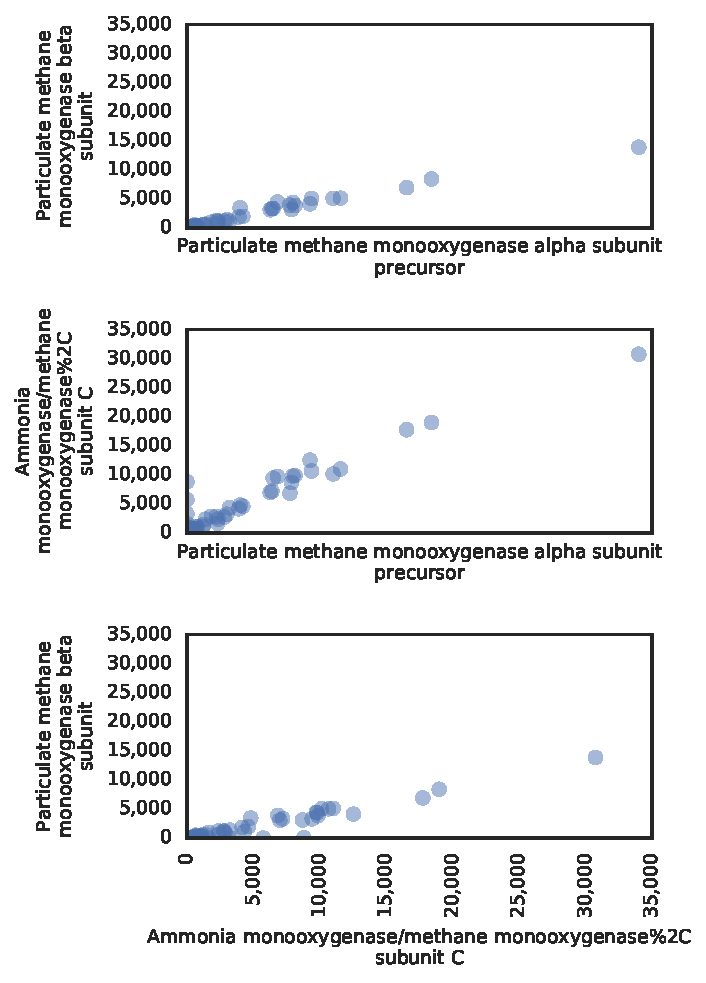
\includegraphics[width=0.7\textwidth]{./tex/chapter3/figures/170402_correlations_between_pMMO_subunits--set3.pdf}
    \begin{singlespace}
    \caption[Demonstration of correlation between \textit{pmo} subniuts in cluster 3]{
        Demonstration of correlation between \textit{pmo} subniuts in cluster 3.}
    \label{fig:pmo_cor3}
    \end{singlespace}
\end{figure}




